\section*{Глава 3. Разработка веб-приложения}
\addcontentsline{toc}{section}{Глава 3. Разработка веб-приложения}
\stepcounter{section}

\subsection{Общая архитектура приложения}

Приложение реализовано как fullstack-проект на платформе Next.js~15 c использованием
парадигмы App Router. Слой представления и серверной логики размещён в едином
репозитории, а в роли источника данных, системы аутентификации и файлового
хранилища выступает облачная платформа Supabase.

Архитектурно приложение разделено на четыре слоя.

\begin{itemize}
    \item \textbf{Серверные компоненты (Server Components)} -- рендерятся
          на сервере, выполняют запросы к базе данных и формируют HTML
          до отправки клиенту. Используются для всех страниц по умолчанию.
    \item \textbf{Клиентские компоненты (Client Components)} -- помеченные
          директивой \texttt{'use client'}. Применяются только там, где
          необходимо состояние и обработка событий: формы, переключатели,
          фильтры, кнопка записи на встречу.
    \item \textbf{Сервисный слой (\texttt{lib/services/})} -- инкапсулирует
          все обращения к Supabase. Компоненты никогда не обращаются к
          базе данных напрямую, что обеспечивает единое место для логики
          доступа к данным и упрощает тестирование.
    \item \textbf{Серверные действия (Server Actions)} -- функции с
          директивой \texttt{'use server'}, используемые для мутаций
          (создание, обновление, удаление). Принимают \texttt{FormData}
          и вызываются непосредственно из форм без отдельного API-маршрута.
\end{itemize}

Структура каталогов проекта представлена в таблице~\ref{tab:structure}.

\begin{table}[h]
\centering
\caption{Структура каталогов приложения}
\label{tab:structure}
\begin{tabular}{|p{5cm}|p{9cm}|}
\hline
\textbf{Путь} & \textbf{Назначение} \\
\hline
\texttt{app/(auth)/} & Страницы регистрации и входа \\
\hline
\texttt{app/(app)/} & Защищённые страницы (каталог, профиль, клубы, встречи, админка) \\
\hline
\texttt{app/api/} & HTTP-маршруты (выгрузка CSV) \\
\hline
\texttt{components/} & Переиспользуемые компоненты интерфейса \\
\hline
\texttt{lib/services/} & Сервисный слой доступа к данным \\
\hline
\texttt{lib/validators/} & Схемы валидации Zod \\
\hline
\texttt{lib/supabase/} & Конфигурация клиентов Supabase \\
\hline
\texttt{supabase/migrations/} & SQL-миграции схемы базы данных \\
\hline
\end{tabular}
\end{table}

\subsection{Реализация модели данных}

Схема базы данных, спроектированная в главе~2, реализована в PostgreSQL
средствами Supabase через систему миграций. Каждая миграция представлена
отдельным SQL-файлом с порядковым номером, что обеспечивает воспроизводимость
схемы на любом окружении и облегчает отслеживание её эволюции.

При создании пользователя через Supabase Auth автоматически срабатывает
триггер, создающий соответствующую запись в таблице \texttt{profiles}
с именем из метаданных регистрации:

\begin{verbatim}
CREATE FUNCTION public.handle_new_user() RETURNS TRIGGER AS $$
BEGIN
  INSERT INTO public.profiles (user_id, name)
  VALUES (NEW.id, COALESCE(NEW.raw_user_meta_data->>'name', ''));
  RETURN NEW;
END $$ LANGUAGE plpgsql SECURITY DEFINER;
\end{verbatim}

Такой подход гарантирует, что у каждого пользователя всегда существует
профиль, и исключает рассогласование между таблицами \texttt{auth.users}
и \texttt{profiles}.

\subsection{Защита данных средствами Row Level Security}

Главным механизмом разграничения доступа в приложении выступает Row Level
Security (RLS) -- средство PostgreSQL, позволяющее ограничивать видимость
и модификацию строк таблицы на уровне самой базы данных. RLS применяется
ко всем запросам независимо от того, из какой части приложения они
сделаны, что исключает класс ошибок, связанных с забытой проверкой
прав в коде сервера.

Для каждой таблицы определены отдельные политики на операции
\texttt{SELECT}, \texttt{INSERT}, \texttt{UPDATE} и \texttt{DELETE}.
Сводка ключевых политик представлена в таблице~\ref{tab:rls}.

\begin{table}[h]
\centering
\caption{Политики RLS для таблиц приложения}
\label{tab:rls}
\begin{tabular}{|p{2.5cm}|p{2.5cm}|p{9cm}|}
\hline
\textbf{Таблица} & \textbf{Операция} & \textbf{Условие} \\
\hline
profiles & SELECT & доступно всем \\
\hline
profiles & UPDATE & владелец профиля или администратор \\
\hline
clubs & SELECT & клуб активен или текущий пользователь -- владелец \\
\hline
clubs & INSERT, UPDATE, DELETE & текущий пользователь -- владелец клуба \\
\hline
meetings & SELECT & доступно всем \\
\hline
meetings & INSERT, UPDATE, DELETE & текущий пользователь -- владелец клуба встречи \\
\hline
registrations & SELECT & собственная запись либо запись на встречу своего клуба \\
\hline
registrations & INSERT & запись создаётся от своего имени \\
\hline
registrations & DELETE & собственная запись \\
\hline
\end{tabular}
\end{table}

Расширенный доступ для администратора реализован отдельной политикой.
Чтобы определить, является ли текущий пользователь администратором,
требуется обратиться к его записи в таблице \texttt{profiles} и
проверить значение поля \texttt{role}. Однако если такую проверку
выполнить непосредственно в политике \texttt{profiles}, возникнет
рекурсия: чтобы прочитать одну строку таблицы, СУБД сначала
обращается к политике, а та, в свою очередь, читает другую строку
той же таблицы. PostgreSQL обнаруживает этот цикл и прерывает
запрос.

Для разрыва цикла проверка роли вынесена в отдельную хранимую
функцию \texttt{public.is\_admin()}, объявленную с признаком
\texttt{SECURITY DEFINER}. Функции с таким признаком исполняются
от имени их владельца и не активируют политики RLS при внутренних
запросах. Политика \texttt{profiles} ссылается на эту функцию вместо
прямого подзапроса, что устраняет рекурсию.

\subsection{Аутентификация и роли пользователей}

Аутентификация реализована средствами Supabase Auth. Регистрация
и вход выполняются по паре <<email -- пароль>>; для повторного
использования сессии Supabase устанавливает зашифрованный
cookie. Серверные компоненты получают текущего пользователя
вызовом \texttt{supabase.auth.getUser()}, который верифицирует
сессию по cookie.

При регистрации в Server Action \texttt{registerAction} последовательно
выполняются:

\begin{enumerate}
    \item Валидация формы схемой \texttt{registerSchema} (Zod) --
          проверка формата email, минимальной длины пароля и совпадения
          поля подтверждения;
    \item Вызов \texttt{supabase.auth.signUp} с передачей имени
          в \texttt{options.data.name} -- его подхватит триггер
          создания профиля;
    \item Детекция повторной регистрации по пустому массиву
          \texttt{identities} -- Supabase не возвращает ошибку при
          дубликате email, поэтому критерий вычисляется вручную;
    \item Перевод сообщения об ошибке Supabase на русский язык
          функцией \texttt{translateAuthError}.
\end{enumerate}

Роли пользователей в системе устроены минимально. В таблице
\texttt{profiles} хранится лишь два значения поля \texttt{role}:
\texttt{member} и \texttt{admin}. Статус организатора, в отличие
от роли, не сохраняется явно -- он определяется наличием хотя бы
одного клуба, в котором \texttt{owner\_id = auth.uid()}. Такое
решение позволяет любому участнику стать организатором без явного
изменения роли и упрощает модель прав.

Блокировка пользователя выражается флагом \texttt{is\_active = false}
в таблице \texttt{profiles}. При следующем переходе по защищённой
странице корневой компонент \texttt{(app)/layout.tsx} проверяет
этот флаг и, в случае блокировки, инициирует выход из системы
и редирект на страницу входа с параметром \texttt{?blocked=1},
по которому отображается соответствующее уведомление.

\subsection{Сервисный слой и серверные действия}

Все обращения к базе данных сосредоточены в модулях каталога
\texttt{lib/services/}. Каждая функция возвращает значение типа
\texttt{Result<T>}, представляющее собой алгебраический тип:

\begin{verbatim}
type Result<T> =
  | { data: T; error: null }
  | { data: null; error: string };
\end{verbatim}

Такой контракт исключает выбрасывание исключений из сервисов и
делает обработку ошибок явной в вызывающем коде. Сводка ключевых
сервисов приведена в таблице~\ref{tab:services}.

\begin{table}[h]
\centering
\caption{Сервисный слой приложения}
\label{tab:services}
\begin{tabular}{|p{4cm}|p{10cm}|}
\hline
\textbf{Модуль} & \textbf{Назначение} \\
\hline
\texttt{auth.ts} & Регистрация, вход, выход, перевод ошибок Auth \\
\hline
\texttt{profiles.ts} & Чтение и обновление профиля, загрузка аватара \\
\hline
\texttt{clubs.ts} & CRUD клубов, получение клубов пользователя \\
\hline
\texttt{meetings.ts} & CRUD встреч, фильтрация каталога, выгрузка по клубу \\
\hline
\texttt{registrations.ts} & Запись и отмена записи, экспорт списка участников \\
\hline
\texttt{admin.ts} & Управление статусом пользователей и клубов \\
\hline
\end{tabular}
\end{table}

Мутации интерфейса выполняются через Server Actions. Действие
получает данные формы, валидирует их, вызывает сервисный слой
и при успехе перенаправляет на следующую страницу либо
обновляет текущую вызовом \texttt{revalidatePath}.

\subsection{Реализация ключевых модулей}

\subsubsection{Каталог встреч и фильтрация}

Каталог встреч (страница \texttt{/meetings}) реализован как серверный
компонент. Параметры фильтрации передаются через query-параметры URL
и парсятся схемой \texttt{meetingFilterSchema}. Это позволяет
сохранять состояние фильтра при обновлении страницы и делиться
ссылкой на конкретную выборку.

Фильтр по уровню CEFR реализован как множественный выбор: пользователь
может одновременно выбрать несколько уровней (например, \texttt{B1}
и \texttt{B2}), и результат включит встречи любого из них. Технически
это реализовано через несколько вхождений параметра \texttt{cefr}
в URL и оператор \texttt{IN} в запросе к базе данных.

Дополнительно каталог отсекает встречи, дата которых уже прошла
($\texttt{date} \geq \texttt{NOW()}$), и встречи скрытых клубов через
inner-join с фильтром \texttt{club.is\_active = true}.
Внешний вид страницы каталога представлен на рисунке~\ref{fig:meetings}.

\begin{figure}[h]
\centering
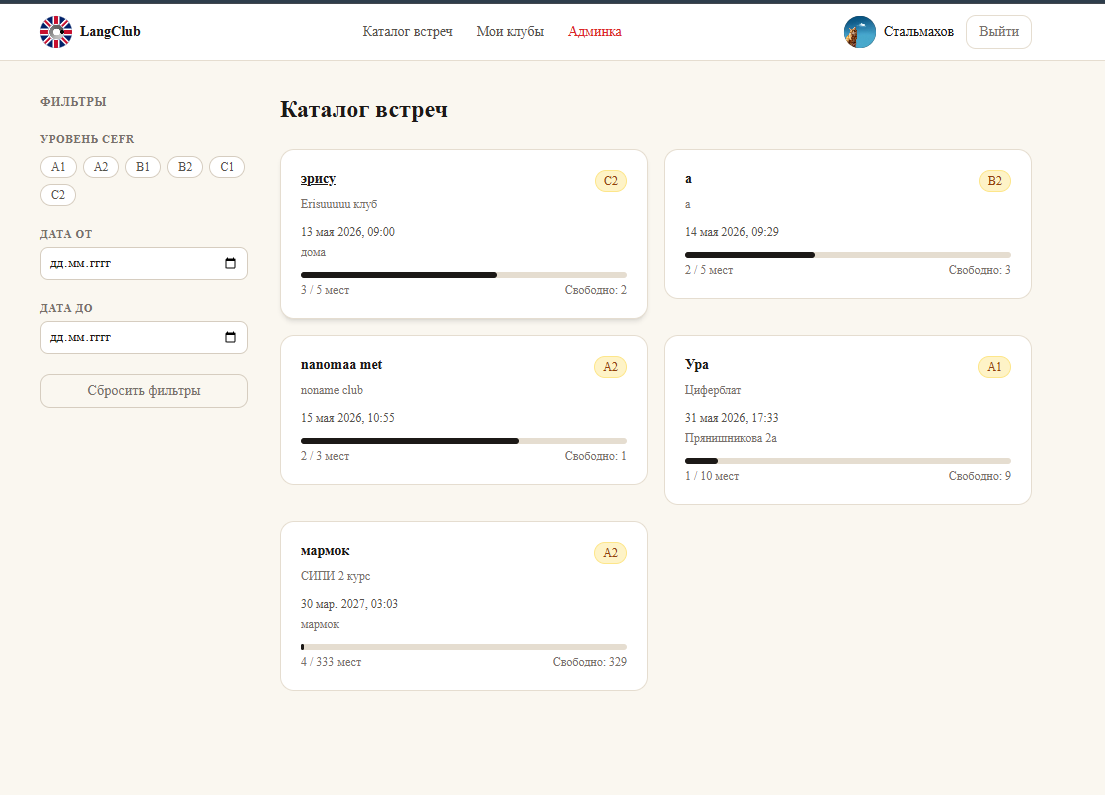
\includegraphics[width=\textwidth]{images/meetings}
\caption{Страница каталога встреч с фильтрами}
\label{fig:meetings}
\end{figure}

\subsubsection{Запись на встречу и защита от перепревышения}

Реализация записи на встречу потребовала особого внимания к
согласованности данных. Первоначальная версия считала количество
занятых мест через агрегатный запрос \texttt{COUNT(*)} к таблице
\texttt{registrations}, однако из-за RLS-политики, скрывающей
чужие записи, обычный пользователь получал нулевой результат и
мог записаться сверх лимита.

Решение состоит из двух частей.

\textbf{Денормализация счётчика.} В таблицу \texttt{meetings}
добавлено поле \texttt{seats\_taken}, инкрементируемое триггером
\texttt{AFTER INSERT OR DELETE ON registrations}. Триггер выполняется
в режиме \texttt{SECURITY DEFINER} и обходит RLS, что делает счётчик
видимым всем пользователям и устраняет лишний запрос на чтение
агрегата.

\textbf{Атомарная проверка при вставке.} Дополнительно создан
триггер \texttt{BEFORE INSERT}, который читает текущие
\texttt{seats\_total} и \texttt{seats\_taken} с блокировкой строки
(\texttt{FOR UPDATE}) и поднимает исключение, если мест не осталось.
Этот уровень защиты исключает гонку при одновременной записи
двух пользователей на последнее место.

\begin{verbatim}
CREATE FUNCTION check_seats_before_registration()
RETURNS TRIGGER SECURITY DEFINER AS $$
BEGIN
  SELECT seats_total, seats_taken INTO v_total, v_taken
  FROM meetings WHERE id = NEW.meeting_id FOR UPDATE;
  IF v_taken >= v_total THEN
    RAISE EXCEPTION 'seats_full';
  END IF;
  RETURN NEW;
END $$ LANGUAGE plpgsql;
\end{verbatim}

Страница отдельной встречи с блоком записи представлена на
рисунке~\ref{fig:meeting}.

\begin{figure}[h]
\centering
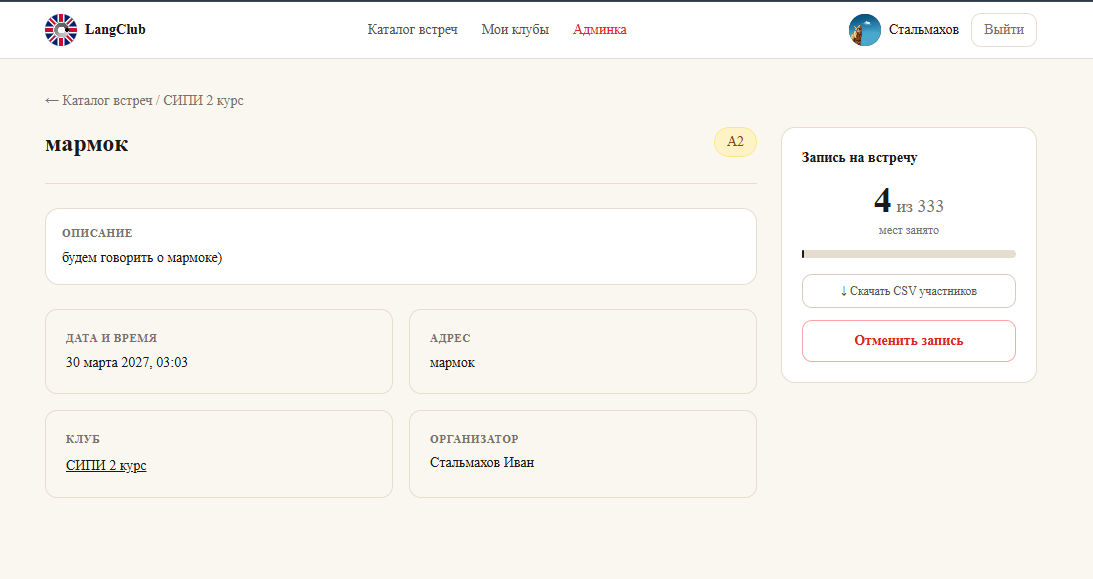
\includegraphics[width=\textwidth]{images/meeting}
\caption{Страница встречи с панелью записи}
\label{fig:meeting}
\end{figure}

\subsubsection{Управление клубами и встречами}

Создание и редактирование клубов и встреч реализовано через формы
с валидацией на стороне клиента (Zod + react-hook-form) и сервера
(повторная валидация в Server Action). Двойная валидация защищает
от обхода клиентских проверок и обеспечивает целостность данных.

Принадлежность клуба определяется полем \texttt{owner\_id},
автоматически проставляемым в момент создания. Все операции
изменения и удаления проверяют это поле и средствами RLS,
и в коде сервиса.

Публичная страница клуба со списком предстоящих встреч представлена
на рисунке~\ref{fig:club}, а панель организатора с управлением
клубами и встречами -- на рисунке~\ref{fig:clubs}.

\begin{figure}[h]
\centering
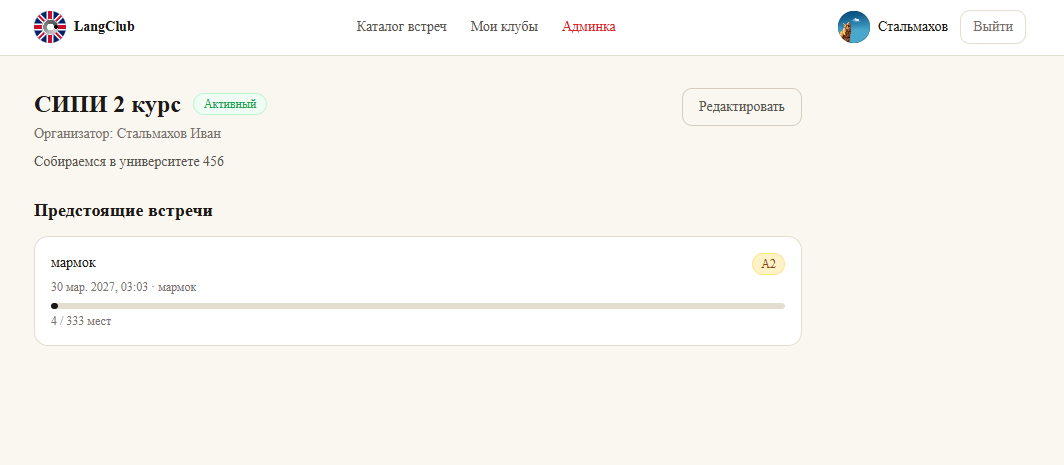
\includegraphics[width=\textwidth]{images/club}
\caption{Страница клуба с предстоящими встречами}
\label{fig:club}
\end{figure}

\begin{figure}[h]
\centering
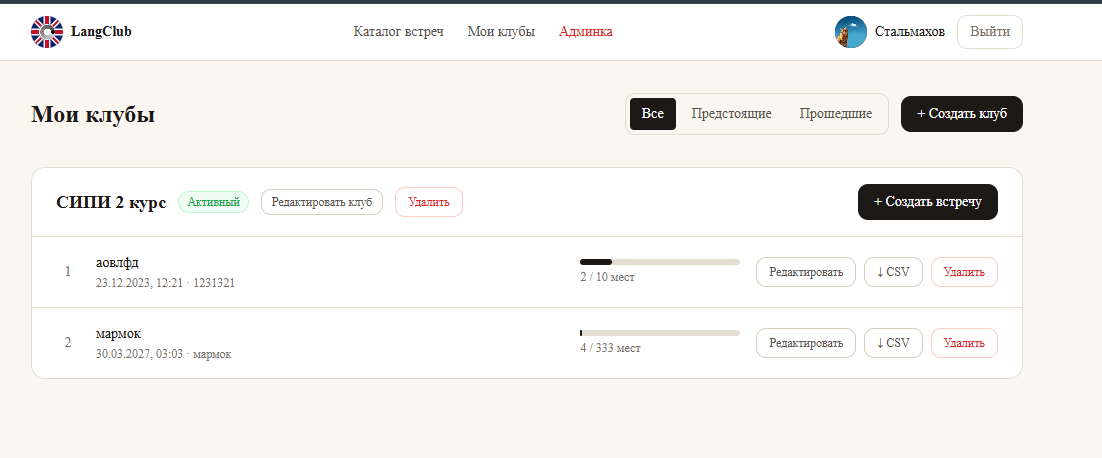
\includegraphics[width=\textwidth]{images/clubs}
\caption{Панель организатора со списком клубов и встреч}
\label{fig:clubs}
\end{figure}

\subsubsection{Загрузка аватара}

Загрузка аватара реализована через Supabase Storage. На странице
профиля файл выбирается через стандартный \texttt{<input type="file">},
после чего клиентский компонент \texttt{ProfileEditor} напрямую
обращается к Supabase Storage из браузера, получает публичный URL
и обновляет поле \texttt{avatar\_url} в профиле. После записи
вызывается \texttt{router.refresh()} для повторного рендера
серверных компонентов (в том числе аватара в навигационной панели).

Доступ к бакету \texttt{avatars} ограничен политиками Storage:
любой пользователь может читать файлы, но загружать или перезаписывать
только в подпапку, имя которой совпадает с его \texttt{user\_id}.
Интерфейс редактирования профиля представлен на рисунке~\ref{fig:profile}.

\begin{figure}[h]
\centering
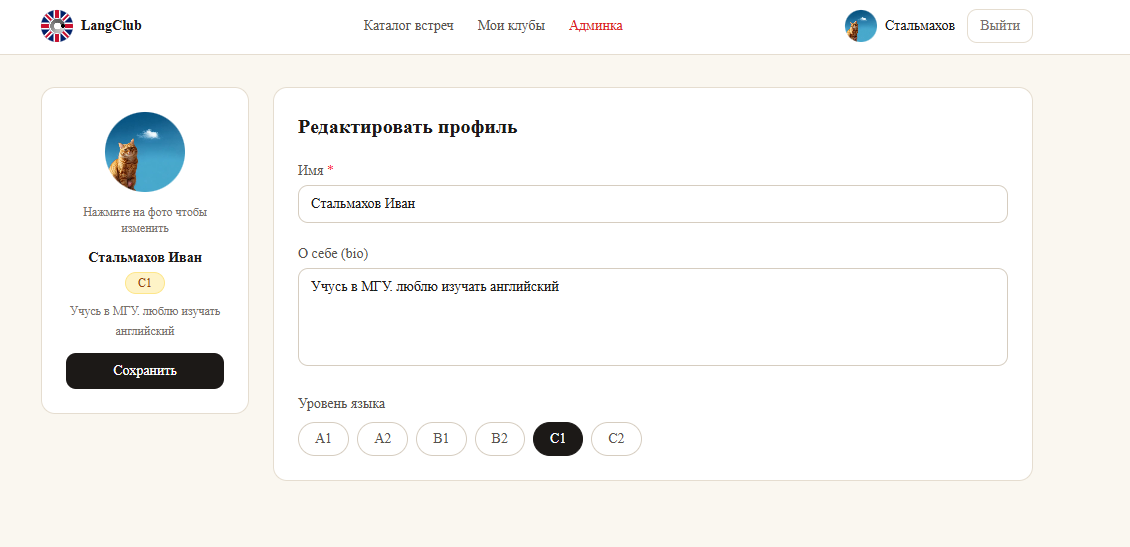
\includegraphics[width=\textwidth]{images/profile}
\caption{Страница редактирования профиля с загрузкой аватара}
\label{fig:profile}
\end{figure}

\subsubsection{Выгрузка списка участников в CSV}

Список участников встречи доступен только владельцу клуба и выгружается
по адресу \texttt{/api/meetings/[id]/export}. В отличие от прочих
мутаций, реализованных через Server Actions, выгрузка файла потребовала
Route Handler, поскольку требует возврата произвольного содержимого
с заголовком \texttt{Content-Disposition}.

Список включает имя участника, уровень CEFR, дату записи и адрес
электронной почты (получаемый через служебный метод
\texttt{auth.admin.listUsers}). Файл формируется согласно RFC~4180
с использованием кодировки UTF-8 и BOM для корректного отображения
в Microsoft Excel.

\subsubsection{Административная панель}

Страница \texttt{/admin} доступна только пользователям с ролью
\texttt{admin}. Корневой компонент маршрута проверяет роль
и при её отсутствии выполняет редирект. Параллельно ссылка
<<Админка>> в навигационной панели отображается только администраторам.

Панель состоит из двух разделов -- управление пользователями
и управление клубами. Для пользователей реализована блокировка
и разблокировка с переключением флага \texttt{is\_active};
администратор не может изменить статус собственной записи.
Для клубов реализовано скрытие и возврат -- скрытый клуб не
отображается в каталоге, его встречи недоступны для записи,
но владелец сохраняет доступ к редактированию. Интерфейс
административной панели представлен на рисунке~\ref{fig:admin}.

\begin{figure}[h]
\centering
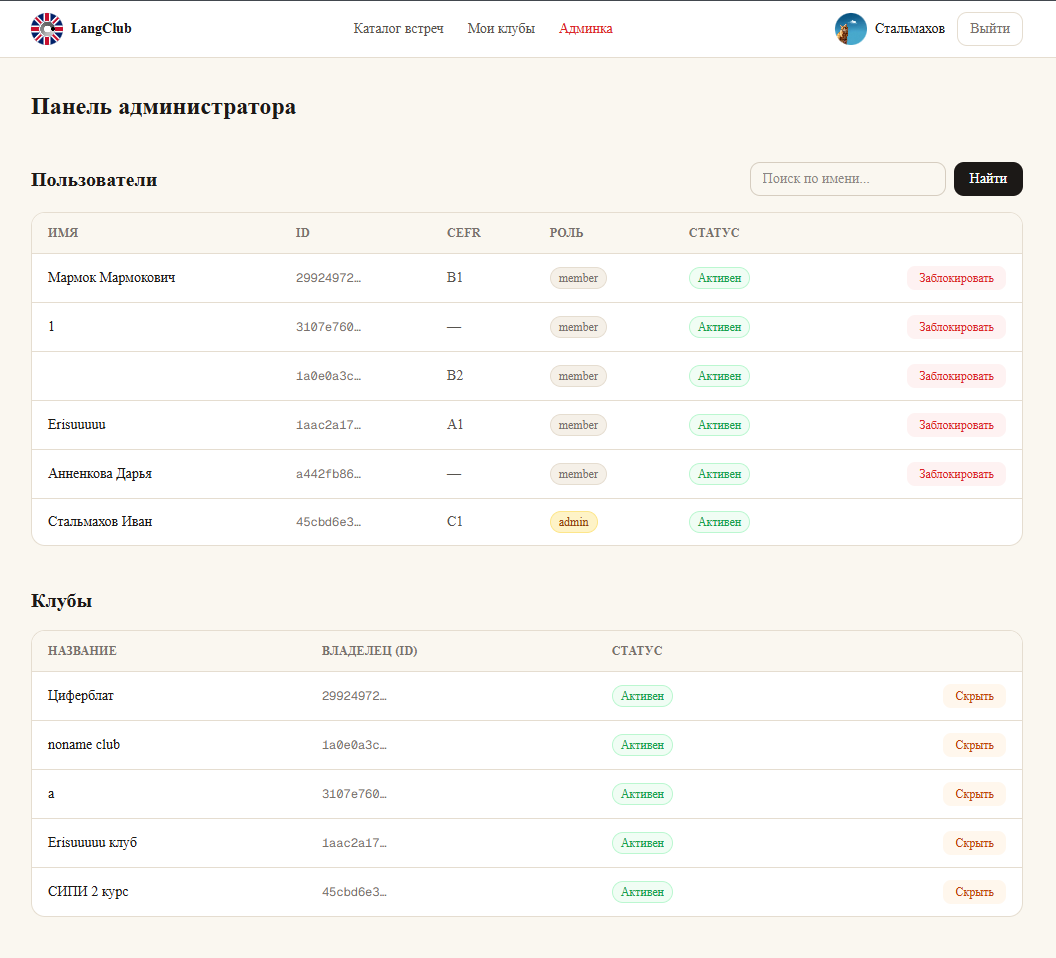
\includegraphics[width=\textwidth]{images/admin}
\caption{Панель администратора с разделами пользователей и клубов}
\label{fig:admin}
\end{figure}

\subsection{Тестирование}

Для верификации ключевых компонентов написаны три типа тестов
(таблица~\ref{tab:tests}).

\begin{table}[h]
\centering
\caption{Покрытие тестами}
\label{tab:tests}
\begin{tabular}{|p{3cm}|p{4cm}|p{8cm}|}
\hline
\textbf{Тип} & \textbf{Фреймворк} & \textbf{Покрываемая логика} \\
\hline
Юнит & Vitest & Валидаторы Zod, форматтеры дат, генератор CSV \\
\hline
Интеграция & Vitest + моки & Сервис записи на встречу: ветки <<занято>>, <<дубликат>>, <<клуб неактивен>> \\
\hline
E2E & Playwright & Полный сценарий: регистрация, создание клуба и встречи, запись, выгрузка CSV \\
\hline
\end{tabular}
\end{table}

Особое внимание уделено сервису \texttt{registrations} как наиболее
ответственному за согласованность данных. Тесты разработаны
в стиле TDD до реализации сервиса, что позволило формализовать
контракт функции через возвращаемый алгебраический тип
\texttt{\{ ok: true \} | \{ ok: false; reason: ... \}}.

\subsection{Деплой приложения}

Готовое приложение развёрнуто на платформе Vercel в режиме production.
Деплой инициируется автоматически при пуше в основную ветку
репозитория GitHub либо вручную командой \texttt{vercel --prod}.

Конфигурация подключения к Supabase передаётся через переменные
окружения, заданные в настройках проекта Vercel. Среди них --
URL проекта Supabase, публичный анонимный ключ для клиента и
сервисный ключ для серверных операций (например, обращения к
\texttt{auth.admin.listUsers} при выгрузке участников).

В результате реализованы все функциональные возможности, заявленные
в главе~2: каталог встреч с фильтрацией, профиль пользователя
с аватаром и уровнем CEFR, CRUD клубов и встреч, запись и отмена
записи, выгрузка списка участников в CSV, административная панель
с модерацией пользователей и клубов.
